\documentclass[11pt]{article}

% arXiv-friendly packages
\usepackage[utf8]{inputenc}
\usepackage[T1]{fontenc}
\usepackage{lmodern}
\usepackage{microtype}
\usepackage{geometry}
\geometry{margin=1in}
\usepackage{graphicx}
\usepackage{booktabs}
\usepackage{array}
\usepackage{amsmath,amssymb}
\usepackage{hyperref}
\usepackage{enumitem}
\usepackage{caption}
\usepackage{multirow}
\usepackage{xcolor}

\hypersetup{
  colorlinks=true,
  linkcolor=blue,
  citecolor=blue,
  urlcolor=blue
}

\title{Simulation-Generated Data for Multimodal Small Language Models:\\
A Constrained-Hardware Recipe for Medical Physics Visual Question Answering}
\author{
  Jaydip Singh\\
  \textit{Independent Researcher}\\
  \texttt{jaydip.singh@gmail.com}
}
\date{\today}

\begin{document}
\maketitle

\begin{abstract}
Multimodal models that answer questions about medical images normally depend on
large, expert-annotated datasets that are costly to build and constrained by
patient privacy. We present a fully reproducible recipe that sidesteps this
bottleneck by training a multimodal small language model (SLM) entirely on
\emph{simulation-generated} data, where exact ground truth is produced
automatically and no human annotation is required. An analytical image simulator
generates positron emission tomography (PET) reconstructions, sinograms, and
phantom diagrams, and---because every physical parameter of each image is
known---emits matching multiple-choice question--answer (QA) pairs directly from
those parameters. The learner is a 23M-parameter model that couples a trainable
convolutional vision encoder and a spatial vision--language projection to a
physics-pretrained decoder-only transformer (TinyLMv3); it is trained end-to-end
on a single Apple~M3~Pro laptop with 18\,GB of unified memory. On a held-out
benchmark of 35{,}596 image--question pairs, the model attains an overall accuracy
of \textbf{43.7\%}, well above a 25\% random baseline and, importantly, above an
image-agnostic text-only baseline (33.3\%)---a control that isolates genuine image
use. Beyond the headline number, we contribute a candid account of the
development trajectory: an initial run scored \emph{below} random ($\sim$11\%),
which we trace to two compounding defects---an answer-scoring bug that measured
answer length rather than content, and a vision pathway that was silently
disabled during training. We describe the diagnosis and the architectural fixes
(a spatial, non-pooling projection and a gradient-enabled encoder) that recovered
real image-grounded performance. A per-task analysis then shows an interpretable
split: the model is strong on global-appearance questions (artifact detection,
tumor presence) and weak on fine spatial localization, pointing to concrete
future work. All code, data generators, and evaluation and diagnostic harnesses
are released to support replication.
\end{abstract}

%----------------------------------------------------------------------
\section{Introduction}
\label{sec:intro}
%----------------------------------------------------------------------

Visual question answering (VQA) asks a model to answer a natural-language
question about an image, and it has matured rapidly from early feature-fusion
systems to today's large vision--language models~\cite{ishmam2025vqasurvey}. In
the medical domain, VQA is especially attractive because it promises accessible
interfaces to imaging data, but it inherits a hard prerequisite: models are
typically trained on large datasets that pair images with expert annotations or
radiology reports~\cite{lin2023medvqasurvey}. Producing such annotations is
expensive, requires scarce clinical expertise, suffers from inter-rater
variability, and is entangled with patient-privacy constraints. Surveys of
medical VQA repeatedly identify data scarcity and annotation cost as the central
obstacles to progress~\cite{lin2023medvqasurvey}, and recent clinician-facing
studies note that dataset quality and provenance are precisely what practitioners
worry about~\cite{jin2025medvqabarriers}.

A growing body of work responds to this bottleneck by training on
\emph{synthetic} data. Generative approaches show that medical vision--language
pre-training on synthetic images can match, and sometimes exceed, training on
real images~\cite{hu2023medvlpsynthetic,liu2024medvlppurelysynthetic}, and
foundation models can now synthesize realistic chest X-rays on
demand~\cite{bluethgen2024chestxray}. These methods, however, rely on large
generative models to \emph{produce} the images and still require care to obtain
labels. Our approach is complementary and deliberately lightweight: rather than
generating photorealistic images from text, we use a compact physics
\emph{simulator} whose parameters are known by construction, so the labels come
for free.

This is the core idea of the paper---an \emph{image simulator as a zero-cost
labeled-data generator}. Because we control every simulation parameter (tumor
count, position, size, uptake ratio, artifact type), we obtain exact ground truth
without any human in the loop and convert it automatically into multiple-choice
QA pairs. The principle mirrors domain randomization in robotics, where training
on procedurally varied simulated data transfers to the real
world~\cite{tobin2017domainrand}; here we apply it to medical-physics imaging. A
compact multimodal model then learns to read these images and answer questions
about them.

At the same time, small language models (SLMs) and small vision--language models
are increasingly viable for low-cost, on-device, and reproducible
research---SmolVLM, for instance, runs a capable multimodal model in under a
gigabyte of GPU memory~\cite{marafioti2025smolvlm}. Yet end-to-end multimodal SLM
\emph{training recipes for constrained hardware} are rarely documented in full.
This paper contributes such a recipe, trained and evaluated entirely on a single
laptop.

We are deliberate about scope and honesty. The simulator used here is an
\textbf{analytical NumPy simulation} (Poisson counting statistics, point-spread
blurring, and a simplified Radon transform for sinograms), \emph{not} a full
Geant4 Monte~Carlo simulation; extending to a Monte~Carlo simulator is left as
future work. The model is small (23M parameters) and runs on a laptop. And rather
than report only a final number, we document the complete development
trajectory---including a phase in which the system scored \emph{below} random due
to two compounding bugs---because that trajectory, and the diagnostics that
resolved it, are among the most transferable parts of the contribution.

Our contributions are:
\begin{enumerate}[leftmargin=*]
    \item A simulation-to-model pipeline that produces unlimited,
    exactly-labeled medical-physics visual QA data with no human annotation.
    \item A 23M-parameter multimodal SLM (trainable CNN encoder + spatial
    vision--language projection + physics-pretrained TinyLMv3) trained
    end-to-end on an 18\,GB laptop.
    \item A rigorous evaluation on 35{,}596 held-out image--question pairs, with a
    per-category and per-image-type breakdown.
    \item A transparent failure analysis: how a below-random result was
    diagnosed and fixed, and where the working model still fails (fine spatial
    localization).
\end{enumerate}

%----------------------------------------------------------------------
\section{Related Work}
\label{sec:related}
%----------------------------------------------------------------------

\paragraph{Medical visual question answering.}
Medical VQA sits at the intersection of medical AI and general VQA: given a
medical image and a clinically relevant question, the system must produce a
plausible answer~\cite{lin2023medvqasurvey}. The broader VQA field has evolved
from hand-engineered feature fusion to large vision--language
models~\cite{ishmam2025vqasurvey}, but medical VQA remains bottlenecked by the
cost and scarcity of expertly annotated data. Recent work also cautions that
technical accuracy alone does not guarantee clinical utility: a survey of
radiologists found limited enthusiasm for current medical-VQA systems, citing
missing patient context and concerns about training-data
provenance~\cite{jin2025medvqabarriers}. Our contribution addresses the data
axis specifically---not by curating more clinical data, but by generating exactly
labeled data from a simulator---while being explicit that our benchmark is
synthetic and not a claim of clinical readiness.

\paragraph{Synthetic and simulation-based training data.}
Training on synthetic data is an increasingly credible strategy in medical
imaging. Hu et al.~\cite{hu2023medvlpsynthetic} replace real images with
synthetic equivalents generated from genuine radiology reports and find that
downstream performance is on par with, or better than, training on real images.
Liu et al.~\cite{liu2024medvlppurelysynthetic} go further, showing that
vision--language pre-training on \emph{purely} synthetic data can outperform
real-data training on zero-shot classification, and that mixing synthetic and
real data helps more still. Generative foundation models can now produce
realistic chest X-rays to mitigate dataset paucity~\cite{bluethgen2024chestxray}.
These methods use large generative networks to synthesize images; our approach
instead uses a lightweight analytical simulator whose parameters directly furnish
the labels---closer in spirit to domain randomization, where procedurally varied
simulation data transfers to real systems~\cite{tobin2017domainrand}.

\paragraph{Vision--language architectures and projections.}
Most modern vision--language models follow a common template: a pretrained vision
encoder, a language model, and a learned \emph{projection} (or connector) that
maps visual features into the language model's embedding space. LLaVA showed that
even a simple connector, trained with visual instruction tuning, yields strong
multimodal ability~\cite{liu2023llava}, and that a two-layer MLP projection with
appropriate data further improves results~\cite{liu2024improved}. The vision
encoder itself is commonly a contrastively trained model such as
SigLIP~\cite{zhai2023siglip,tschannen2025siglip2}. Our design follows this
template but at miniature scale and with a domain-specific twist: because our
images are rendered PET/sinogram/phantom scenes rather than natural photographs,
we train a small convolutional encoder from scratch, and---critically---we retain
one projected token per spatial patch rather than pooling, so that spatial
information survives into the language model.

\paragraph{Small and efficient multimodal models.}
There is rising interest in compact vision--language models for on-device and
resource-constrained deployment. SmolVLM demonstrates capable multimodal
reasoning in under a gigabyte of GPU memory and argues that na\"ively shrinking
large-model design choices is wasteful~\cite{marafioti2025smolvlm}. Our work
occupies the far end of this spectrum: a sub-25M-parameter multimodal model
trained \emph{and} evaluated on a single laptop, prioritizing reproducibility and
transparent analysis over raw capability.

\paragraph{Relationship to our prior work.}
This paper extends a text-only physics SLM---a 23M-parameter decoder-only
transformer using rotary position embeddings (RoPE)~\cite{su2021rope}, RMS
normalization~\cite{zhang2019rmsnorm}, and SwiGLU feed-forward
layers~\cite{shazeer2020glu}, pretrained on physics arXiv papers with a 32K
byte-pair-encoding tokenizer~\cite{sennrich2016bpe}---by adding a vision pathway.
Because the language backbone and tokenizer are reused unchanged, the present work
isolates the contribution of the visual modality on top of an otherwise fixed
language model.

%----------------------------------------------------------------------
\section{Data Generation}
\label{sec:data}
%----------------------------------------------------------------------

The value of a simulator-as-labeler is that it inverts the usual annotation
problem: instead of showing an image to an expert and asking what is in it, we
first \emph{decide} what is in the image (the parameters) and then render it.
Every label is therefore correct by construction, arbitrarily many examples can
be produced, and the full distribution of cases---including rare ones---is under
our control. This subsection describes the generator; the next describes how QA
pairs are derived from its parameters.

\subsection{Analytical image simulator}

The generator produces three image types with an analytical NumPy pipeline. We
emphasize that this is a first-order, physically motivated approximation rather
than a Monte~Carlo transport simulation; it is fast enough to generate tens of
thousands of images on a laptop, which is what the training recipe requires.

\begin{itemize}[leftmargin=*]
    \item \textbf{PET reconstructions.} An activity map (brain/lung/body
    background with optional tumors of controlled position, diameter, and SUV
    ratio) is corrupted with Poisson counting noise and blurred by a
    point-spread function, then normalized.
    \item \textbf{Sinograms.} A simplified forward (Radon-like) projection of a
    phantom, with Poisson noise and optionally injected detector artifacts
    (gap, ring, or scatter).
    \item \textbf{Phantom diagrams.} Schematic cross-sections showing the
    detector ring, body outline, and tumor placements.
\end{itemize}

\subsection{Automatic question--answer generation}

Because every simulation parameter is known, we template multiple-choice QA pairs
directly from ground truth, with distractor options drawn from the same value
space so that chance performance is well defined (one correct option among
several). The questions span four categories that probe different visual
competencies: \emph{tumor\_detection} (is a lesion present, how many),
\emph{localization} (which quadrant, what diameter), \emph{parameter} (e.g.\ SUV
ratio, anatomical region), and \emph{quality} (e.g.\ which detector artifact is
present). This categorization matters for analysis: detection and quality
questions can often be answered from global image appearance, whereas
localization requires resolving \emph{where} something is---a distinction that
turns out to explain the model's per-task performance
(Section~\ref{sec:results}). In total we generate 10{,}000 images yielding
35{,}596 QA pairs (Table~\ref{tab:data}).

\begin{table}[t]
\centering
\caption{Generated dataset composition (10{,}000 images, 35{,}596 QA pairs).}
\label{tab:data}
\begin{tabular}{lr}
\toprule
\textbf{Breakdown} & \textbf{Count} \\
\midrule
Image type: PET reconstruction & 24{,}741 \\
Image type: sinogram           & 5{,}749 \\
Image type: phantom            & 5{,}106 \\
\midrule
Category: tumor\_detection     & 14{,}957 \\
Category: parameter            & 10{,}800 \\
Category: localization         & 6{,}580 \\
Category: quality              & 3{,}259 \\
\bottomrule
\end{tabular}
\end{table}

%----------------------------------------------------------------------
\section{Model and Training}
\label{sec:model}
%----------------------------------------------------------------------

\subsection{Architecture}

The multimodal model concatenates vision tokens with text token embeddings and
feeds the combined sequence to the language model for next-token prediction:
\[
[\underbrace{\text{vision tokens}}_{64}\;\;|\;\;\underbrace{\text{text tokens}}_{\le 128}] \rightarrow \text{TinyLMv3} \rightarrow \text{answer logits}.
\]

\begin{itemize}[leftmargin=*]
    \item \textbf{Vision encoder.} A from-scratch convolutional network maps a
    $128\times128$ image to an $8\times8$ grid of 64 patch features. It is
    trained (not frozen) so it learns features specific to PET/sinogram imagery.
    \item \textbf{Spatial projection.} Following the connector template of
    LLaVA-style models~\cite{liu2023llava,liu2024improved}, a per-patch MLP maps
    each patch feature into the language embedding space; we add a learned
    positional embedding per patch so the language model can tell patches apart.
    The result is 64 vision tokens, one per spatial location. Critically, this
    projection preserves spatial structure---an earlier design that
    global-average-pooled all patches into a single vector destroyed it and made
    the model effectively blind (Section~\ref{sec:failure}).
    \item \textbf{Language model.} TinyLMv3, a 23M-parameter decoder-only
    transformer using RoPE~\cite{su2021rope}, RMSNorm~\cite{zhang2019rmsnorm}, and
    SwiGLU~\cite{shazeer2020glu}, pretrained on physics arXiv text and reused here
    unchanged as the language backbone.
\end{itemize}

\subsection{Two-stage training}

Training proceeds in two stages on a single Apple~M3~Pro (18\,GB), auto-selecting
the MPS backend:
\begin{enumerate}[leftmargin=*]
    \item \textbf{Alignment.} The language model is frozen; the CNN encoder and
    projection are trained so vision tokens align with the language embedding
    space.
    \item \textbf{Instruction tuning.} The encoder and projection continue
    training while the language model adapts to the visual QA task.
\end{enumerate}

Answers are scored by teacher-forced log-probability ranking. For each candidate
option, we append the option text to the question, run a single forward pass, and
sum the model's log-probabilities of the answer tokens (each predicted from the
position immediately before it), then normalize by the number of answer tokens.
The option with the highest length-normalized log-probability is selected. This
avoids free-form generation and gives a deterministic, comparable score across
options; as Section~\ref{sec:failure} details, getting the token bookkeeping of
this procedure exactly right---accounting for both subword boundaries and the
prepended vision tokens---turned out to be essential.

%----------------------------------------------------------------------
\section{Results}
\label{sec:results}
%----------------------------------------------------------------------

\begin{table}[t]
\centering
\caption{Overall accuracy on the full held-out multiple-choice benchmark
(35{,}596 QA pairs).}
\label{tab:overall}
\begin{tabular}{lc}
\toprule
\textbf{System} & \textbf{Accuracy} \\
\midrule
Random baseline                 & 25.0\% \\
Text-only heuristic (no image)  & 33.3\% \\
Most-frequent-answer baseline   & 34.1\% \\
\midrule
\textbf{PhysVision-SLM (23M, ours)} & \textbf{43.7\%} \\
\bottomrule
\end{tabular}
\end{table}

\begin{table}[t]
\centering
\caption{Accuracy breakdown over the full 35{,}596-pair benchmark ($n$ per row).
The model excels on global-appearance tasks and struggles with fine spatial
localization.}
\label{tab:breakdown}
\begin{tabular}{lcr}
\toprule
\textbf{By category} & \textbf{Accuracy} & \textbf{$n$} \\
\midrule
quality (artifact type)   & 68.6\% & 3{,}259 \\
tumor\_detection          & 64.9\% & 14{,}957 \\
parameter                 & 23.7\% & 10{,}800 \\
localization              & 16.1\% & 6{,}580 \\
\midrule
\textbf{By image type} & & \\
\midrule
sinogram                  & 81.4\% & 5{,}749 \\
pet\_reconstruction       & 36.9\% & 24{,}741 \\
phantom                   & 34.3\% & 5{,}106 \\
\bottomrule
\end{tabular}
\end{table}

\begin{figure}[t]
    \centering
    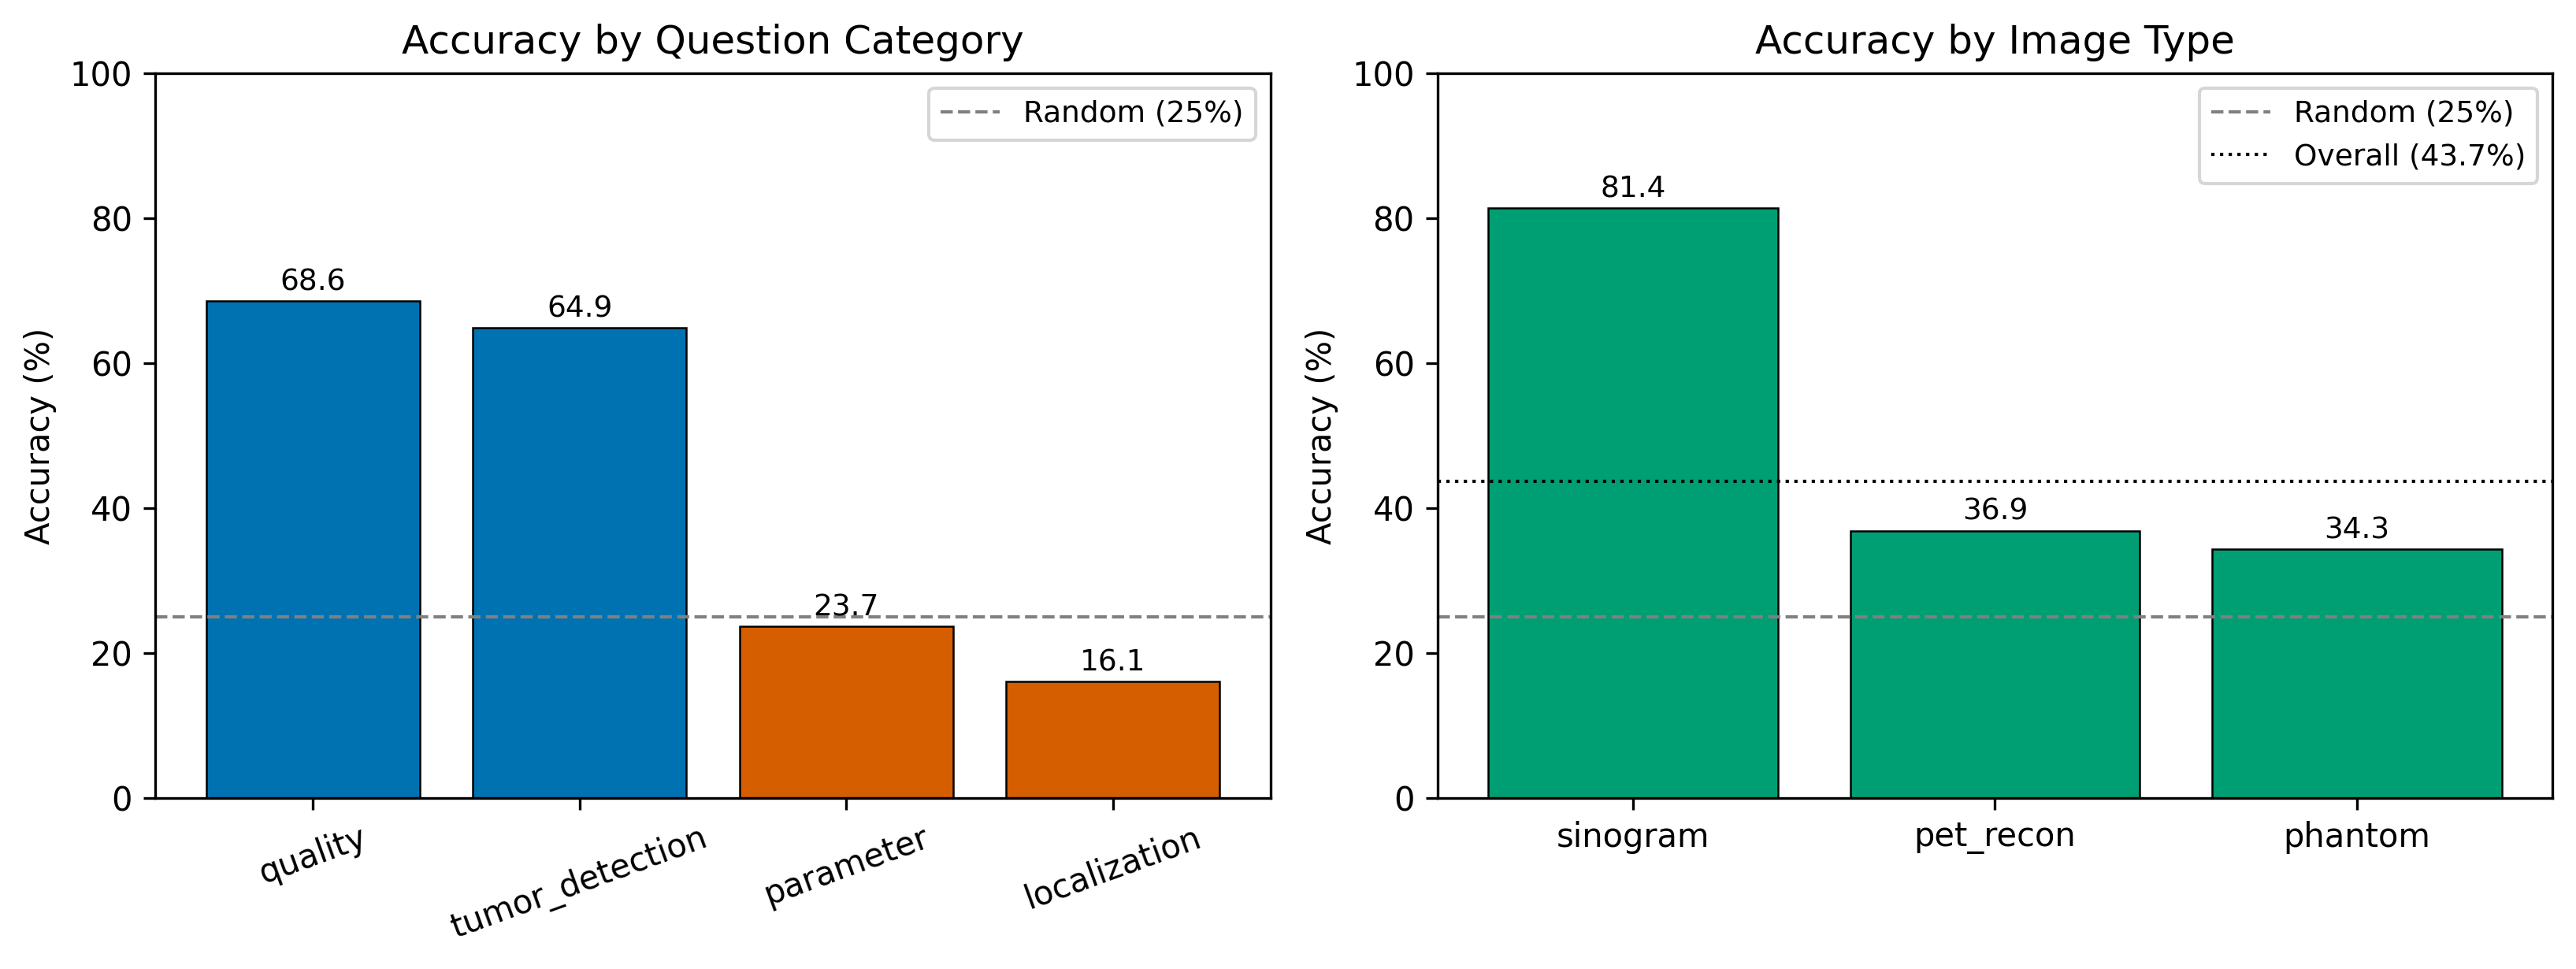
\includegraphics[width=\linewidth]{figure_results.png}
    \caption{Accuracy by question category (left) and image type (right) on the
    full 35{,}596-pair benchmark. Bars above the dashed random line (25\%)
    indicate genuine image-grounded performance; the model is strong on
    global-appearance tasks (sinogram artifacts, tumor presence) and at or below
    random on fine spatial localization.}
    \label{fig:results}
\end{figure}

The model reaches \textbf{43.7\%} overall on the full benchmark, well above the
25\% random baseline and above both the most-frequent-answer (34.1\%) and
text-only (33.3\%) baselines. The text-only baseline is the key control: a model
that ignored the image could not exceed it, so the $\sim$10-point margin over
33.3\% is attributable to genuine image use. This is corroborated by a
counterfactual check in which replacing the real image with a blank image
substantially changes the model's per-option scores on 20/20 sampled questions.

The per-task breakdown (Table~\ref{tab:breakdown}) is interpretable.
\emph{Sinogram} questions are easiest (81.4\%): artifacts and high-uptake lesions
produce distinctive global texture the encoder reads well. \emph{Quality} and
\emph{tumor\_detection} are also strong (68.6\%, 64.9\%), as presence/appearance
questions depend on global image statistics. In contrast, \emph{parameter}
(23.7\%) and especially \emph{localization} (16.1\%) are at or below random:
quadrant and diameter questions demand precise spatial reasoning that an
$8\times8$ patch grid and a small CNN do not resolve.

%----------------------------------------------------------------------
\section{Failure Analysis}
\label{sec:failure}
%----------------------------------------------------------------------

We report the full trajectory because it is the most transferable part of this
work. An initial end-to-end run scored \textbf{below random} ($\sim$11\%), with
an impossible signature: the \emph{parameter} category scored exactly 0.0\% over
10{,}800 questions, and options that tokenized to the same length received
byte-identical scores. Two compounding causes were identified:

\begin{enumerate}[leftmargin=*]
    \item \textbf{Answer-scoring bug.} The evaluation tokenized the prompt and
    the answer separately and computed a token offset from the mismatched
    boundaries; with subword tokenization this measured answer \emph{length}
    rather than answer content. The fix tokenizes prompt$+$answer once and scores
    the answer span as a strict suffix, accounting for the vision-token prefix.
    \item \textbf{Silently disabled vision pathway.} The trainable CNN encoder
    was executed under a no-gradient context and was frozen in both training
    stages, so it never left random initialization; and the projection
    global-average-pooled all patches into a single vector, destroying spatial
    information. The fixes enable encoder gradients, train the encoder, and
    replace the pooling projection with a spatial (per-patch) projection.
\end{enumerate}

After the fixes, a counterfactual ``blank-image'' test confirmed the vision
pathway was live (large score deltas on all sampled questions), and the corrected
evaluation recovered the genuine performance reported above. We stress that the
below-random result was an artifact of measurement and wiring, not of the
modeling idea; distinguishing the two required a targeted diagnostic rather than
further training.

%----------------------------------------------------------------------
\section{Limitations}
\label{sec:limitations}
%----------------------------------------------------------------------

\begin{itemize}[leftmargin=*]
    \item \textbf{Analytical, not Monte~Carlo, simulation.} Images are generated
    analytically, not with Geant4; the sim-to-real gap to clinical scanners is
    untested.
    \item \textbf{Fine localization is weak.} Quadrant/size questions score at or
    below random; the current encoder resolution is the likely bottleneck.
    \item \textbf{Internal benchmark only.} Evaluation is on held-out synthetic
    data from the same generator; no external clinical validation is claimed.
    \item \textbf{Small model, narrow domain.} Results should not be extrapolated
    beyond this simulated setting.
\end{itemize}

%----------------------------------------------------------------------
\section{Conclusion}
\label{sec:conclusion}
%----------------------------------------------------------------------

We showed that a physics image simulator can serve as a zero-cost labeled-data
generator for training a compact multimodal SLM, and that such a model---23M
parameters, trained on a single laptop---answers simulated medical-physics visual
questions well above random and above image-agnostic baselines, with a clear,
interpretable split between global-appearance tasks (strong) and fine spatial
localization (weak). Equally, we documented how an initial below-random result
arose from an evaluation bug and a disabled vision pathway, and how targeted
diagnosis---rather than more compute---recovered a genuine result. Future work
includes higher-resolution encoders for localization, a stronger (e.g.\ SigLIP)
frozen encoder in a larger configuration, Geant4-based simulation, and external
validation on real scans.

\section*{Code and Data Availability}
All code, the data generator, training and evaluation scripts, and the
smoke-test and diagnostic tools are released at
\url{https://github.com/JaydipSingh/physvision-slm}.

\section*{Acknowledgements}
The author thanks Linkan Kumbhar for early assistance with the Rust tokenizer
used by the language backbone.

\bibliographystyle{plain}
\bibliography{references}

\end{document}
